\documentclass[prodmode]{acmsmall}

% Package to generate and customize Algorithm as per ACM style
\usepackage[ruled]{algorithm2e}
\usepackage[MeX]{polski}
\usepackage[utf8]{inputenc}
\renewcommand{\algorithmcfname}{ALGORYTM}
\SetAlFnt{\small}
\SetAlCapFnt{\small}
\SetAlCapNameFnt{\small}
\SetAlCapHSkip{0pt}
\IncMargin{-\parindent}

% Document starts
\begin{document}

% Page heads
\markboth{Konrad Gądek}{Porównanie wydajności LinuxThreads i NPTL}

% Title portion
\title{Porównanie wydajności LinuxThreads i Native POSIX Thread Library}
\author{Konrad Gądek
\affil{Akademia Górniczo-Hutnicza}}

\begin{abstract}
Empiryczne prawo Moore'a, tj. obserwacja, że ilość tranzystorów w procesorach podwaja się co określony okres czasu, powoli się załamuje. Problemem stają się ograniczenia wynikające z obecnie wykorzystywanej architektury komputerów oraz wykorzystywanych technologii produkcji. Jednym z rozwiązań tego problemu jest użycie kilku procesorów w jednej jednostce obliczeniowej. By jednak efektywnie wykorzystać ten fakt, aplikacje muszą być pisane w sposób umożliwiający wykorzystanie posiadania wielu rdzeni. Obecnie wykorzystuje się ku temu dwa mechanizmy -- mechanizm procesów i wątków. Wątki od procesów różnią się tym, że w czasie ich tworzenia nie jest kopiowana pamięć aplikacji przez co są znacząco wydajniejsze. Sprawia to jednak pewne problemy, gdyż konieczna jest np. synchronizacja wątków czy sztuczne wymuszanie atomowości pewnych operacji. Mimo tych problemów, użycie wątków jest opłacalne. Procesory wielordzeniowe stają się de facto standardem, coraz częściej wykorzystuje się ,,farmy komputerów'' (tzw. ,,cloud computing'') a także przeprowadza się obliczenia na procesorach GPU, które posiadają setki niezależnych jednostek obliczeniowych. Mimo, że w wielu zastosowaniach wydajność nie ma dużego znaczenia, w obliczeniach numerycznych czy przy tworzeniu systemów operacyjnych zagadnienie to jest kluczowe dla sukcesu produktu. W wypadku systemów operacyjnych rodziny GNU/Linux najbardziej znane są dwie implementacje wątków: LinuxThreads oraz nowsza Native POSIX Thread Library. W tym artykule postaram się sprawdzić, która z nich jest wydajniejsza oraz opracuję API upraszczające korzystanie z mechanizmu wątków w większości wypadków.
\end{abstract}

\maketitle

\section{Wprowadzenie}
Jądro Linux zaczęło wspierać wątki w wersji 1.3.56\cite{mimuw:linux} i od tego czasu nastąpił znaczący rozwój idei wielowątkowości. Obecnie wykorzystywana implementacja -- Native POSIX Thread Library -- zastąpiła LinuxThreads w jądrze 2.6 i następnych. Stworzona przez developerów Red Hata implementacja NPTL -- podobnie jak poprzedniczka -- używa procesów do abstrakcji wątków na poziomie jądra\cite{wiki:ntpl}, jednak z założenia miała odświeżyć i zwiększyć wydajność całego podsystemu\cite{redhat:nptl}.

%\begin{figure}
%\centerline{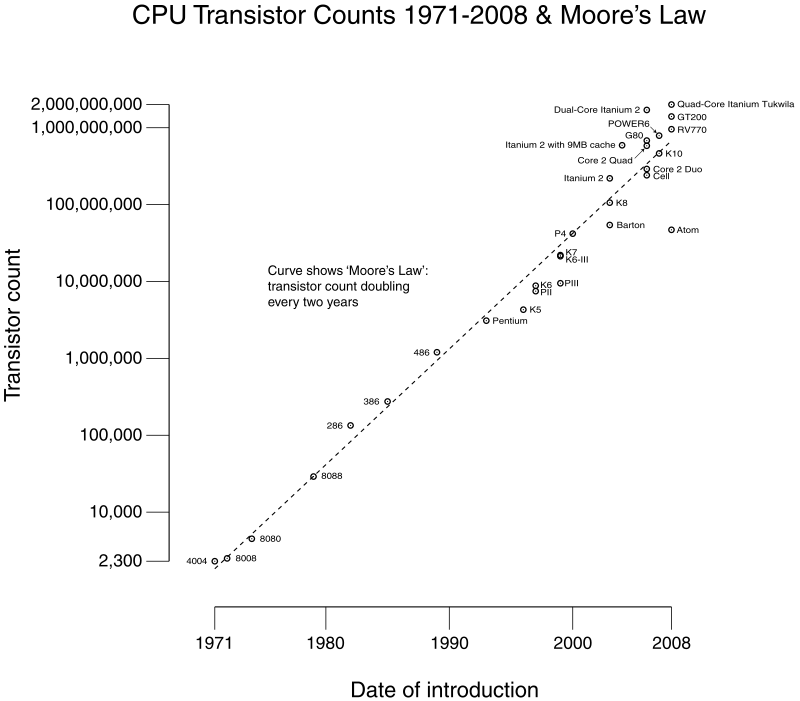
\includegraphics{img/moore.svg}}
%\caption{Ilustracja prawa Moore'a -- ilość tranzystorów procesorów na przebiegu lat.}
%\label{fig:moore}
%\end{figure}

\section{Testy wydajności}

\subsection{Rozważania wstępne}
By stwierdzić, czy NPTL jest faktycznie szybszy od LinuxThreads, należy starannie sprawdzić najważniejsze lub wręcz wszystkie funkcje, jakie udostępniają wątki, pod kątem wydajności. Książka Mitchella\cite{mitchell:advlinuxprog} przestawia wszystkie najważniejsze mechanizmy wątków. Są to:
\begin{itemize}
\item Tworzenie, łączenie i anulowanie wątków
\item Przekazywanie i zwracanie danych z funkcji
\item Ustalanie sekcji krytycznych w wątkach
\item Synchronizacja wątków: muteksy, semafory, zmienne warunkowe
\item Przesyłanie sygnałów między wątkami
\item Zmienne wątków
\end{itemize}

\subsection{Platforma testowa}
Do testów wykorzystałem komputer z procesorem Intel Core i3 wyposażonym w dwa rdzenie i technologię Hyper Threading, 2GB pamięci RAM i macierzą dwóch dysków SATA (połączonych w software'owy RAID 1 -- mirroring). Dla własnej wygody, testowane systemy zainstalowałem na maszynie wirtualnej (Oracle VirtualBox 4.0.8) działającej pod systemem operacyjnym Windows 7 x86-64. Warto podkreślić fakt, że aby umożliwić systemom--gościom korzystanie z wielu rdzeni komputera, należało zmienić domyślne ustawienia programu VirtualBox. By nie testować kolejnych wersji kompilatora GCC -- którego wydajność ulegała znacznej zmianie wraz z kolejnymi wersjami -- na każdym systemie zainstalowałem wersję 4.6.0 tego kompilatora.

\subsection{Tworzenie i łączenie wątków}
Testy mechanizmu tworzenia wątków jest trywialne, wystarczy porównać czasy tworzenia i łączenia pewnej ilości wątków. Możliwe są dwa scenariusze takiego testu: pierwszy (algorytm~\ref{alg:threadcreate1}) tworzy zadaną z góry ilość wątków a następnie oczekuje na ich zamknięcie każdego z nich, drugi scenariusz (algorytm~\ref{alg:threadcreate2}) przewiduje tworzenie i oczekiwanie na zamyknięcie wątku zadaną ilość razy. Warto podkreślić fakt, że drugi program jest praktycznie sekwencyjny, gdyż w jednej chwili działa jedynie jeden wątek roboczy, a wątek główny znajduje się w stanie oczekiwania na jego zakończenie.

\begin{algorithm}[t]
\SetAlgoNoLine
\KwIn{$\alpha$ -- ilość wątków do utworzenia}
\KwOut{Czas wykonania programu}
\For{$i \leftarrow 1 \ldots \alpha$} {
	Stwórz wątek \#$i$\;
}
\For{$i \leftarrow 1 \ldots \alpha$} {
	Poczekaj na zakończenie wątku \#$i$\;
}
\caption{Test tworzenia wątków 1}
\label{alg:threadcreate1}
\end{algorithm}

\begin{algorithm}[t]
\SetAlgoNoLine
\KwIn{$\alpha$ -- ilość wątków do utworzenia}
\KwOut{Czas wykonania programu}
\For{$i \leftarrow 1 \ldots \alpha$} {
	Stwórz wątek \#$i$\;
	Poczekaj na zakończenie wątku \#$i$\;
}
\caption{Test tworzenia wątków 2}
\label{alg:threadcreate2}
\end{algorithm}

Dla każdego z tych testów warto rozważyć kilka podprzypadków. Pierwszy z nich zakłada, że wątek nie wykonuje żadnej pracy i kończy działanie w momencie rozpoczęcia. Drugi przypadek zakłada obliczanie silnii (algorytm~\ref{alg:silnia}), czyli wykorzystanie funcji obciążającej jedynie CPU. W trzecim wypadku warto sprawdzić wydajność stosu funkcji, dlatego doskonała do tego celu będzie funkcja Ackermanna\footnote{Nie warto rozważać wywołań rekurencyjnych w osobnych wątkach -- program taki bardzo szybko natrafia na ograniczenia maksymalnej ilości wątków} (algorytm~\ref{alg:ackermann}):
\[
	A(m,n) = \left\{
		\begin{array}{ll}
			n+1 & \textrm{gdy $m=0$}\\
			A(m-1, 1) & \textrm{gdy $m>0$ i $n=0$}\\
			A(m-1, A(m, n-1)) & \textrm{gdy $m>0$ i $n>0$} 
		\end{array}
	\right.
\]
W czwartym przypadku warto sprawdzić, jak efektywne są operacje na pamięci. Tutaj można wykorzystać algorytm KMP\cite{knuth:kmp} wywołany jednocześnie na tych samych danych.

Należy uważać, by kompilator nie zoptymalizował wywołania prostych funkcji, dlatego nie używałem flagi \verb+-O2+.

\begin{algorithm}[t]
\SetAlgoNoLine
\KwIn{$x$}
\KwOut{$x!$}
$result \leftarrow 1$\;
\Repeat{$x > 0$} {
	$result \leftarrow result \times x$\;
	$x \leftarrow x - 1$
}
\caption{Wyznaczanie wartości silni}
\label{alg:silnia}
\end{algorithm}


\begin{algorithm}[t]
\SetAlgoNoLine
\KwIn{$x$}
\KwOut{$x!$}
$result = 1$\;
\Repeat{$x > 0$} {
	$result = result \times x$\;
	$x = x - 1$
}
\caption{Wyznaczanie wartości funkcji Ackermanna}
\label{alg:ackermann}
\end{algorithm}


%\begin{algorithm}[t]
%\SetAlgoNoLine
%\KwIn{Node $\alpha$'s ID ($ID_{\alpha}$), and node $\alpha$'s
%neighbors' IDs within two communication hops.}
%\KwOut{The frequency number ($FreNum_{\alpha}$) node $\alpha$ gets assigned.}
%$index$ = 0; $FreNum_{\alpha}$ = -1\;
%\Repeat{$FreNum_{\alpha} > -1$}{
%        $Rnd_{\alpha}$ = Random($ID_{\alpha}$, $index$)\;
%        $Found$ = $TRUE$\;
%        \For{each node $\beta$ in $\alpha$'s two communication hops
%    }{
%     $Rnd_{\beta}$ = Random($ID_{\beta}$, $index$)\;
%      \If{($Rnd_{\alpha} < Rnd_{\beta}$) \text{or} ($Rnd_{\alpha}$ ==
%          $Rnd_{\beta}$ \text{and} $ID_{\alpha} < ID_{\beta}$)\;
%      }{
%        $Found$ = $FALSE$; break\;
%      }
%        }
%     \eIf{$Found$}{
%           $FreNum_{\alpha}$ = $index$\;
%         }{
%           $index$ ++\;
%     }
%      }
%\caption{Frequency Number Computation}
%\label{alg:one}
%\end{algorithm}




% Bibliography
\bibliographystyle{acmsmall}
\bibliography{bibliografia}

\end{document}

